\chapter{Overview of Technologies}

We provide a brief theoretical overview of the technologies used in this work and other important related methods that preceded them.
Additionally, a summary of the relevant libraries and frameworks used for the implementation of the experiments is also provided.


\section{Transformers}

\textbf{Transformers} \parencite{AttentionIsAllYouNeed} are a modern type of neural network architecture that has achieved remarkable results in various machine learning tasks, particularly in natural language processing (NLP), computer vision and sequence modeling, often outperforming previous SOTA solutions.
While the original transformer architecture was designed for NLP tasks, it has since been adapted and extended to a wide range of applications, including time series classification - the focus of this work.

While~\cite{AttentionIsAllYouNeed} introduce both encoder and decoder blocks in their work, for our task of time-series classification mainly the encoder blocks are relevant.

\subsection{High level workflow}

At a high level, a transformer processes an input sequence through the following steps:

\begin{enumerate}
    \item \textbf{Tokenize the input.}
    Split the input into a sequence of $n$ tokens.

    \item \textbf{Embed the tokens.}
    Map each token to a vector in the model's representation space, optionally adding positional information so the model can distinguish token order:
    \[
        X_0 \in \mathbb{R}^{n \times d_{\mathrm{model}}}.
    \]

    \item \textbf{Apply $L$ transformer layers.}
    For each layer $l = 1, \dots, L$, the model updates the token representations using attention and a feed-forward network:
    \begin{enumerate}
        \item \textbf{Multi-head self-attention.}
        Each token attends to other tokens in the sequence, producing context-aware representations:
        \[
            H_l = \mathrm{Attention}_l(X_{l-1}),
            \qquad
            H_l \in \mathbb{R}^{n \times d_{\mathrm{model}}}.
        \]

        \item \textbf{Residual connection and layer normalization.}
        The attention output is added back to the layer input, then normalized:
        \[
            U_l = \mathrm{LayerNorm}(X_{l-1} + H_l),
            \qquad
            U_l \in \mathbb{R}^{n \times d_{\mathrm{model}}}.
        \]

        \item \textbf{Feed-forward network (FFN).}
        A position-wise feed-forward network further transforms each token representation:
        \[
            F_l = \mathrm{FFN}_l(U_l),
            \qquad
            F_l \in \mathbb{R}^{n \times d_{\mathrm{model}}}.
        \]

        \item \textbf{Second residual connection and layer normalization.}
        The FFN output is added back to its input and normalized again:
        \[
            X_l = \mathrm{LayerNorm}(U_l + F_l),
            \qquad
            X_l \in \mathbb{R}^{n \times d_{\mathrm{model}}}.
        \]
    \end{enumerate}

    \item \textbf{Obtain final contextualized representations.}
    After the final layer, the model produces
    \[
        X_L \in \mathbb{R}^{n \times d_{\mathrm{model}}},
    \]
    where each token representation now encodes information about both the token itself and its surrounding context.

    \item \textbf{Generate task-specific outputs.}
    The final representations are mapped to outputs depending on the task:
    \begin{enumerate}
        \item \textbf{Sequence classification:}
        Select or pool one representation from $X_L$ (for example, a designated classification token), then apply a linear layer and softmax to produce class probabilities.

        \item \textbf{Next-token prediction:}
        Project each token representation in $X_L$ to vocabulary logits
        \[
            Z \in \mathbb{R}^{n \times |\mathcal{V}|},
        \]
        then apply softmax to obtain a probability distribution over the next token.
    \end{enumerate}
\end{enumerate}

\begin{figure}[!htbp]
    \centering
    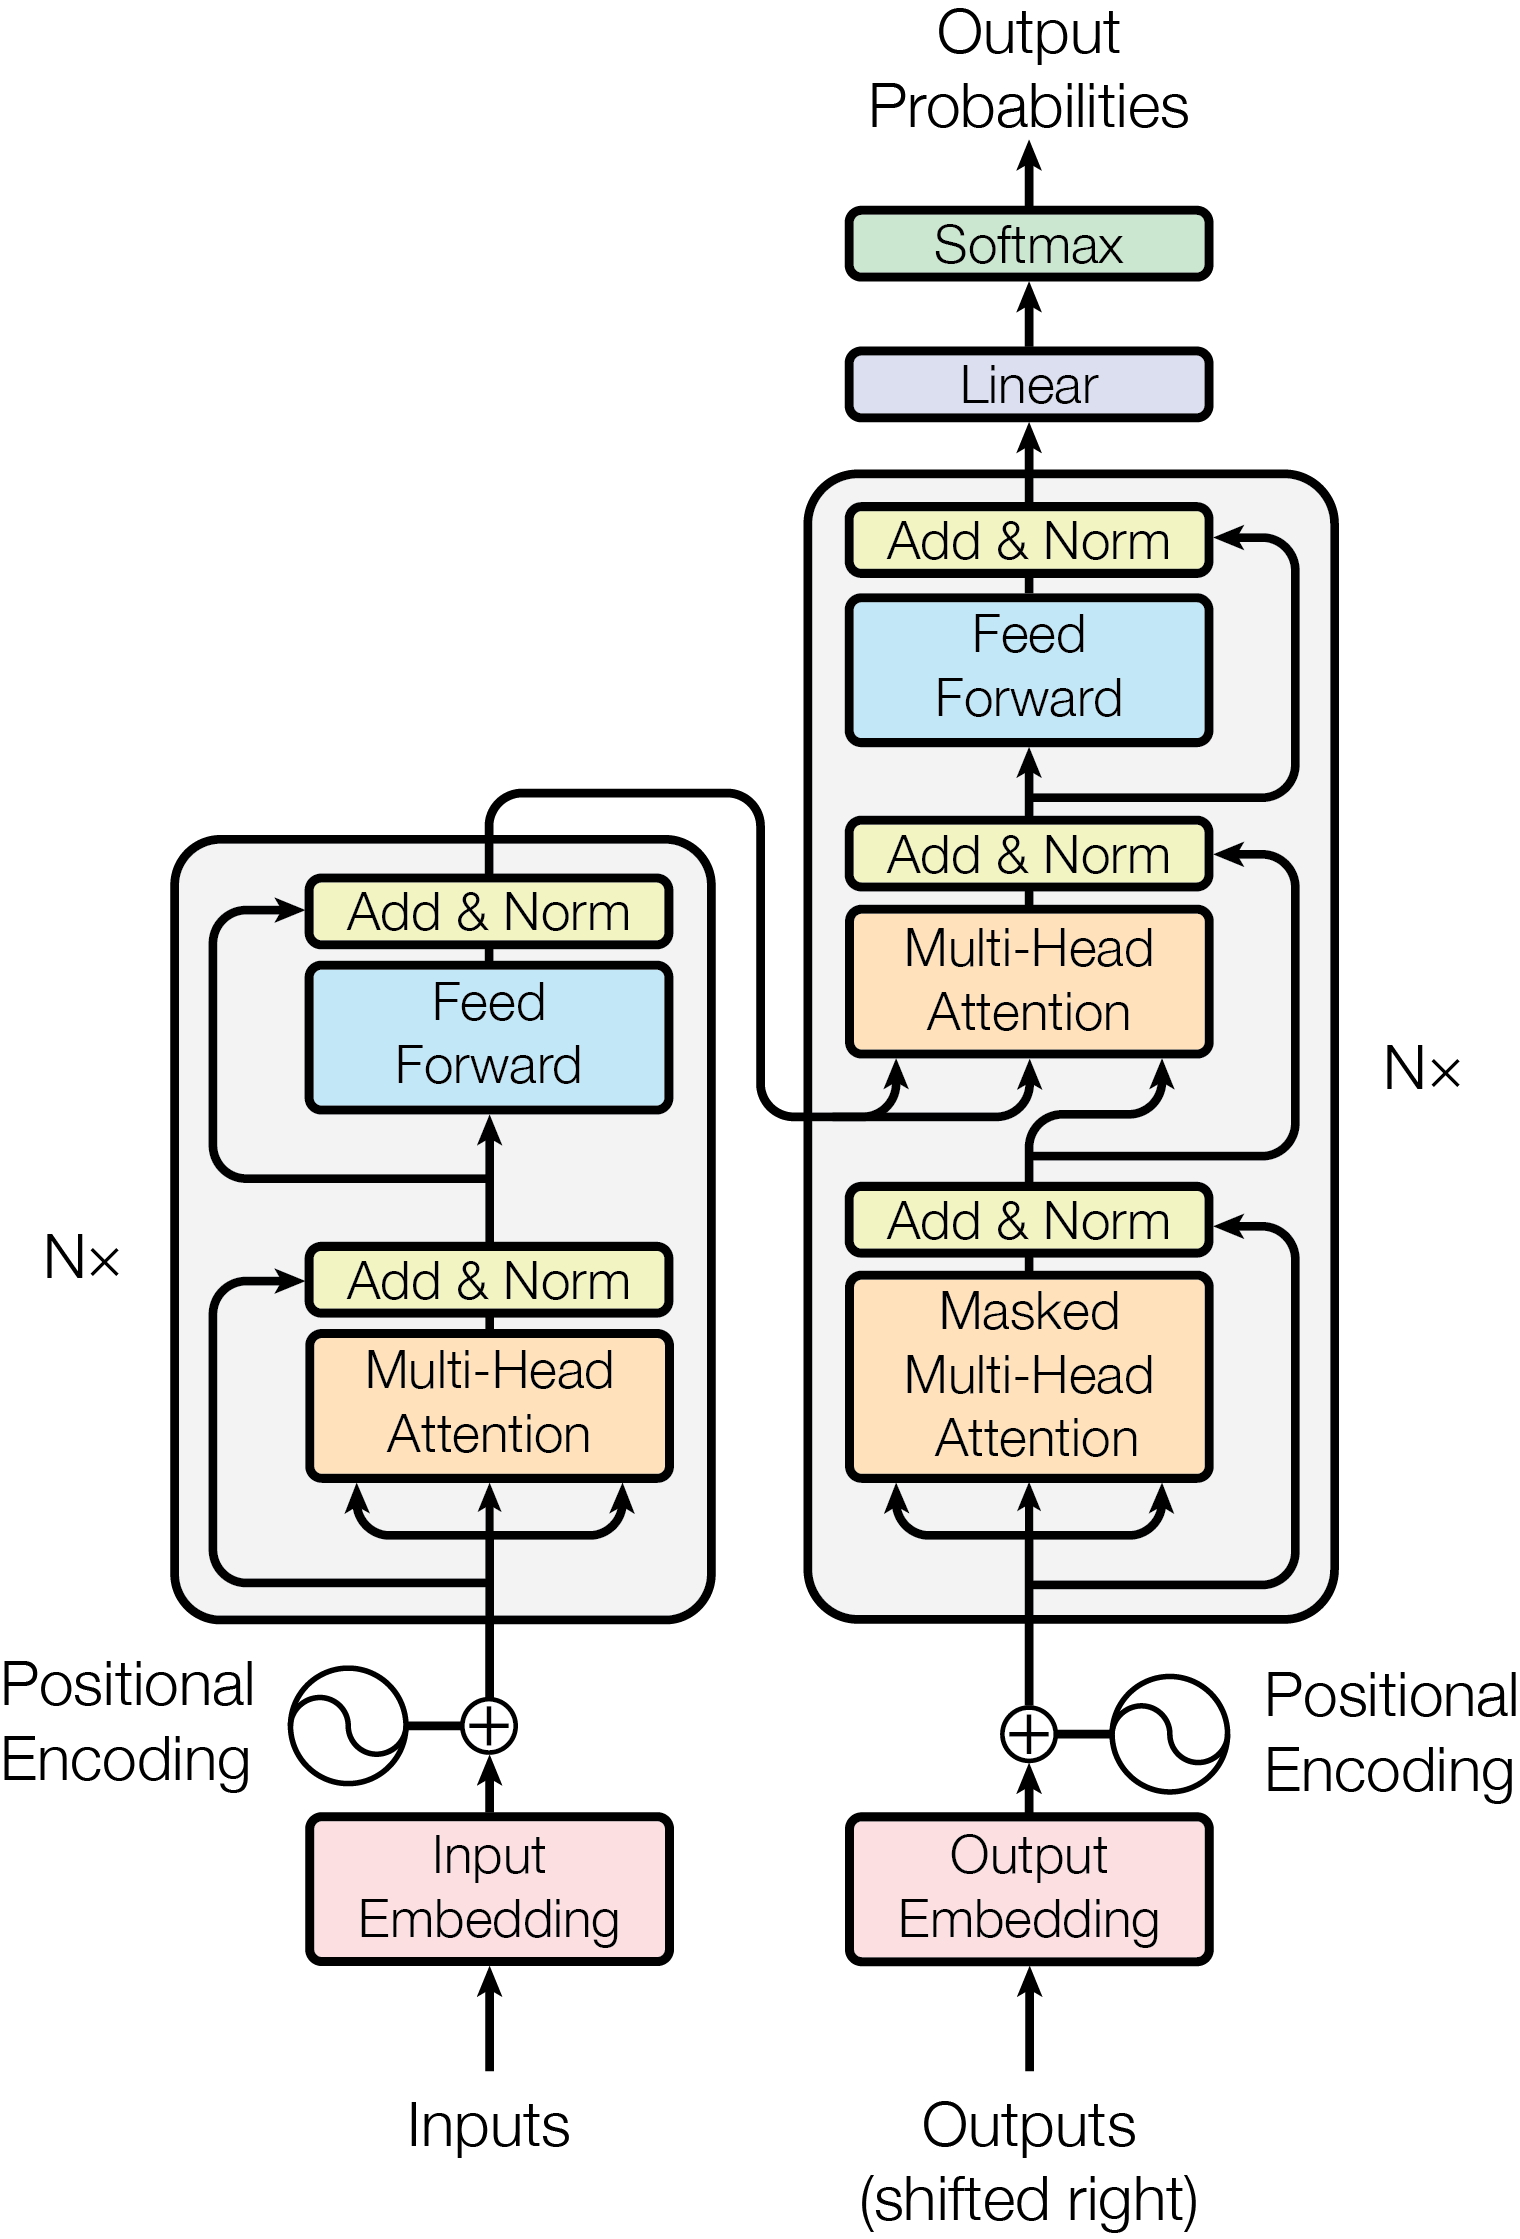
\includegraphics[width=\linewidth]{images/03_transformer}
    \caption[Transformer architecture]{Transformer architecture \parencite{AttentionIsAllYouNeed}}
    \label{fig:03_transformer}
\end{figure}

\subsection{Input and multimodality}

Historically, LLMs were primarily designed for NLP tasks, but recent advancements have led to the development of \textbf{multimodal models} that can process and generate data across multiple modalities, such as text, images and audio.

At its core, a multimodal model extends the transformer architecture to handle different kinds of input data by utilizing modality-specific encoders and decoders, as well as cross-modal attention mechanisms.

For our use-case of time-series classification, we can treat the data as a 1D input of dimension $d_{\mathrm{in}}$ and implement a custom \textbf{tokenizer} and \textbf{embedding layer}.

\subsubsection{Tokenizer}

\textbf{Tokenizer} is responsible for converting the raw data into a sequence of $n$ tokens of dimension $d_{\mathrm{token}}$ that can be processed by the embedding layer.

\subsubsection{Embedding Layer}

\textbf{Embedding Layer} projects the tokens into the model's representation space of dimension $d_{\mathrm{model}}$.

In the case of a fixed vocabulary of size $\mathcal{V}$ (i.e.\ LLMs), a parameter matrix $W \in \mathbb{R}^{\mathcal{V} \times d_{\mathrm{model}}}$ is learned during the training.
This allows the embedding layer to learn unique embedding for each token independently.

When the input is more diverse (i.e.\ time series) a learnable embedding layer is added instead.
Since this approach uses a linear projection it requires the tokens to be vectors of the same dimension $d_{\mathrm{token}}$.

\subsubsection{Positional Embeddings}

\textbf{Positional Embeddings} inject positional information into the embedding vector, allowing the transformer to distinguish token order during \textbf{Self-Attention}.

Two kinds of positional embeddings are commonly used

\begin{itemize}
    \item \textbf{Learned positional embeddings}: a parameter matrix $P \in \mathbb{R}^{L_{\mathrm{max}} \times d_{\mathrm{model}}}$ is learned during training.
    Each row of $P$ then corresponds to a different position in a sequence limited to length $L_{\mathrm{max}}$.
    \item \textbf{Sinusoidal positional embeddings} \parencite{AttentionIsAllYouNeed}: For position $p$ and dimension $i$
    \begin{align*}
        PE(pos, 2i) = \mathrm{sin} \left(\frac{p}{10000^{2i / d_{\mathrm{model}}}}\right) \\
        PE(pos, 2i + 1) = \mathrm{cos} \left(\frac{p}{10000^{2i / d_{\mathrm{model}}}}\right)
    \end{align*}
\end{itemize}

\subsection{Self-Attention Mechanism}

\textbf{Self-Attention} is an essential mechanism that allows the transformer model to add contextual information from the whole sequence to the evaluated token\footnote{Tokens are the elementary blocks of the input sequence (i.e. words)}.
This allows all tokens to influence the meaning of each other token, regardless of their distance in the sequence itself.
This is especially useful when long-range relationships in the data are important.

\bigskip

\noindent For a layer $l$, given weight matrices $W_Q, \, W_K, \, W_V \in \mathbb{R}^{d_{\mathrm{model}} \times (h d_{\mathrm{head}})}$ and a layer input $X_{l-1}$, the multi-head attention self-attention $H_l$ is calculated the following way

        {\setlength{\jot}{1em}
\begin{enumerate}
    \item \textbf{Compute $Q$ (queries), $K$ (keys), $V$ (values)} for each head $i \in \{1, 2, \dots, h\}$
    \[
        Q_i = X_{l-1}W^{(i)}_Q,
        \qquad
        K_i = X_{l-1}W^{(i)}_K,
        \qquad
        V_i = X_{l-1}W^{(i)}_V,
    \]
    $W_Q^{(i)}, \, W_K^{(i)}, \, W_V^{(i)} \in \mathbb{R}^{d_{\mathrm{model}} \times d_{\mathrm{head}}}$ are the weight matrices for the head $i$ and $Q_i, \, K_i, \, V_i \in \mathbb{R}^{n \times d_{\mathrm{head}}}$.
    \item \textbf{Compute attention scores $S_i$ for each head $i$}
    \[
        S_i = \frac{Q_{i}K_{i}^{\top}}{\sqrt{d_{\mathrm{head}}}},
        \qquad S_i \in \mathbb{R}^{n \times n},
    \]
    Each entry of $S_i$ then measures how strongly a token attends to another.
    \item \textbf{Apply row-wise softmax} to obtain \textbf{Attention weights}
    \[
        A_i = \mathrm{softmax}(S_i),
        \qquad
        A_i \in \mathbb{R}^{n \times n}.
    \]
    Each row of $A_i$ then sums to 1.
    \item \textbf{Compute weighted sum of the value vectors}
    \[
        Z_i = A_i V_i,
        \qquad
        Z_i \in \mathbb{R}^{n \times d_{\mathrm{head}}},
    \]
    This gives a context-aware representation based on all tokens in the sequence.
    \item \textbf{Concatenate the weighted sums} $Z_i$ of all $h$ heads
    \[
        Z = \mathrm{Concatenate}(Z_1, Z_2, \dots, Z_h),
        \qquad
        Z \in \mathbb{R}^{n \times (h d_{\mathrm{head}})},
    \]
    In most implementations $h d_{\mathrm{head}} = d_{\mathrm{model}}$.
    \item \textbf{Project back to model dimension} (output projection)
    \[
        H_l = ZW_O,
        \qquad
        H_l \in \mathbb{R}^{n \times d_{\mathrm{model}}},
    \]
    $W_O \in \mathbb{R}^{(h d_{\mathrm{head}}) \times d_{\mathrm{model}}}$ is the output projection weight matrix.

\end{enumerate}
}

\subsection{Feed-Forward Network (FFN)}

\textbf{Feed-Forward Network} is the second main component of a transformer layer which independently transforms each token after attention mixes information between tokens.
It usually consists of a two-layer MLP which projects the token vector into some higher dimensional hidden space of dimension $d_{\mathrm{ff}}$ and then back into the model space of dimension $d_{\mathrm{model}}$. \parencite{AttentionIsAllYouNeed}

This projection, combined with an activation function $\phi$\footnote{ReLU and GELU are commonly used activation functions in FFNs} gives the model additional capacity to express nonlinear combinations of features.
It has been shown that the mixing of feature information in FFN translates to the transformer's ability to learn complex patterns in the data. \parencite{Dai2022}
\bigskip

\noindent After $\textbf{Attention}$ and $\textbf{LayerNorm}$ a vector $u \in \mathbb{R}^{d_{\mathrm{model}}}$ is obtained.

\[
    F = \mathrm{FFN}_{\phi}(u) = W_2 \phi(W_1 u + b_1) + b_2,
\]

\smallskip

\noindent $W_1 \in \mathbb{R}^{d_{\mathrm{model}} \times d_{\mathrm{ff}}}, \, W_2 \in \mathbb{R}^{d_{\mathrm{ff}} \times d_{\mathrm{model}}}$.

\subsubsection{Gated FFNs}

\textbf{Gated FFNs} are used in modern transformer architectures, especially newer LLMs.
They allow richer feature interactions than traditional FFNs by enabling multiplicative scaling of features in addition to plain activation in a special layer - \textbf{Gated Linear Unit} (GLU). \parencite{Dauphin2017}

\bigskip

\noindent For a feature vector $u \in \mathbb{R}^{d_{\mathrm{model}}}$ a Gated FFN with activation function $\phi$ looks like

\[
    \mathrm{GLU}_{\phi}(u) = (W_v u + b_v) \odot \phi(W_g u + b_g)
\]


\[
    \mathrm{GATED\_FFN}_{\phi}(u) = W_o GLU_{\phi}(u) + b_o
\]

\smallskip

\noindent $W_v, W_g \in \mathbb{R}^{d_{\mathrm{model}} \times d_{\mathrm{ff}}}, \, W_o \in \mathbb{R}^{d_{\mathrm{ff}} \times d_{\mathrm{model}}}$  and $\odot$ represents element-wise multiplication.

\subsection{Computational Performance}
Since most operations in the transformer rely on matrix multiplication, they can be efficiently computed in parallel on modern GPUs and other specialized hardware (i.e.\ AWS Trainium\footnote{https://aws.amazon.com/ai/machine-learning/trainium/}).
Efficient parallelization and breakthroughs in hardware have been key factors in the success of transformer models, enabling them to be trained on massive volumes of data and achieve SOTA performance across various tasks.


\section{Large Language Models}

\textbf{Large Language Models} (LLMs) are transformer-based models that are used for a wide range of NLP tasks, including text generation, translation, summarization and question answering.
LLMs typically consist of billions of parameters and are trained on massive datasets containing trillions of tokens, which allows them to learn complex language patterns and perform well on diverse tasks.

It has been shown that LLMs can be adapted to non-NLP tasks, such as time series classification, by treating the input data as a sequence of tokens and \textbf{fine-tuning} the pretrained model on the specific task.
This approach leverages the powerful representation learning capabilities of LLMs, allowing them to solve tasks commonly considered outside the scope of language understanding.

\subsection{Fine-Tuning}

\textbf{Fine-tuning} is the process of modifying the weights of a pretrained model to adapt it to a specific task or domain.
This is typically done by initializing the model with the pretrained weights and then training it on a smaller dataset, modifying the original weights to better fit the new task while retaining the general knowledge learned during pretraining. \parencite{Howard2018}

Full fine-tuning is however both computationally and memory intensive, making it infeasible for small research teams with limited resources.
This has led to the development of more efficient fine-tuning methods that utilize different techniques to drastically reduce the costs associated with full fine-tuning while still achieving comparable performance. \parencite{Han2024}

Update of a weight matrix $W \in \mathbb{R}^{p \times q}$ during full fine-tuning can be expressed as

\[
    W' = W + \alpha \Delta W,
\]

$\alpha \in \mathbb{R}$ is a scaling factor and $\Delta W$ is the update matrix that is learned during fine-tuning.

\subsubsection{Low Rank Adaptation (LoRA)}\label{subsubsec:03-lora}

\textbf{Low Rank Adaptation} is a fine-tuning method that reduces the number of trainable parameters by decomposing the weight update matrices into matrices of rank $r$.
It has been empirically shown that \textbf{LoRA} can consistently achieve comparable performance to full fine-tuning while reducing the memory overhead by up to $2 / 3$ if $r \ll d_{\mathrm{model}}$.
It has been also shown $r \geq 8$ is sufficient to match the performance of full fine-tuning in most cases. \parencite{Hu2021}

\subsubsection{QLoRA}

\textbf{QLoRA} is a further improvement over \textbf{LoRA} that uses a quantized \footnote{a technique where the model's weights are converted to lower-precision representation to save memory} version of the pretrained model and memory paging which further reduces the memory overhead.
Quantization to 4 bits and 8 bits is commonly used in \textbf{QLoRA}, which reduces the amount of memory used to load the model itself by $75\%$ and $50\%$ respectively. \parencite{Dettmers2023}

\begin{figure}[!htbp]
    \centering
    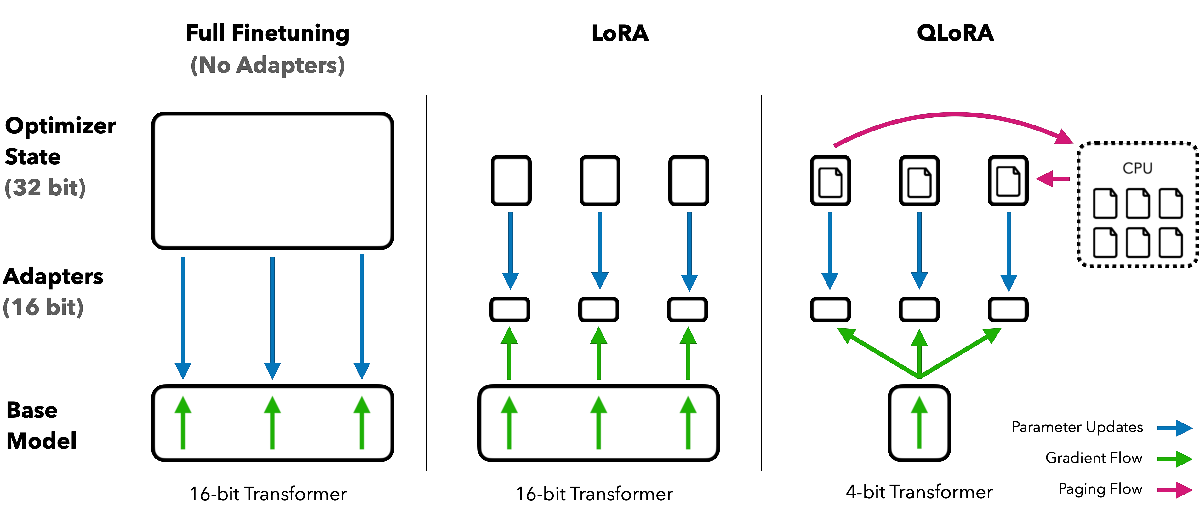
\includegraphics[width=\linewidth]{images/03_qlora}
    \caption[Comparison of the fine-tuning methods]{Comparison of the fine-tuning methods \parencite{Dettmers2023}}
    \label{fig:03_qlora}
\end{figure}


\section{Other Technologies}

\subsection{PyTorch}

\textbf{PyTorch}\footnote{https://pytorch.org/} is an open-source Python machine learning framework, originally developed by Meta, that is mainly designed for deep learning, including computer vision and natural language processing.
PyTorch implements many commonly used components of neural networks, such as linear layers, transformer layers, loss functions and optimizers.
These components enable fast design, training and deployment of models in a unified environment.

Broad GPU support is another great feature of PyTorch that allows most code to utilize GPU acceleration for faster model training and inference with minimal changes to the existing code, making its use fairly straightforward.
Multiple different GPU frameworks are supported, like NVIDIA CUDA, AMD ROCm and Intel XPU, with NVIDIA CUDA being the most widely used and optimized.

\subsection{HuggingFace}

\textbf{HuggingFace}\footnote{https://huggingface.co} is an open-source platform and community focused on machine learning.
It provides multiple tools and libraries for easier training, fine-tuning and distribution of models.

\subsubsection{HuggingFace Hub}

\textbf{HuggingFace Hub}\footnote{https://huggingface.co/docs/hub/index} is an online platform that allows the hosting of git repositories, models, datasets and hosting of demo apps (spaces), additionally to hosting, it also supports discussion and collaboration of users.
Currently, around 2 million models 500 thousand datasets are publicly available on the Hub, with many more being stored in private repositories.

Other HuggingFace libraries can then interface with the Hub, allowing the user to seamlessly access the hosted models and datasets through the code without the need for manual downloading.

\subsubsection{Transformers}

\textbf{Transformers}\footnote{https://huggingface.co/docs/transformers/en/index} is a library that contains many useful tools for interfacing with different machine learning models, providing a unified framework for both training and inference.
Transformers can be used to load models and datasets directly from the Hub and also contain useful abstractions, such as the Trainer class which implements a unified interface for passing parameters, monitoring and saving checkpoints during training.

\subsubsection{PEFT}

\textbf{PEFT}\footnote{https://huggingface.co/docs/peft/index} (Parameter-Efficient Fine-Tunig) is a library that implements efficient fine-tuning mechanisms for large pretrained models, such as \textbf{LoRA} and \textbf{QLoRA}.


\section{Experimental Environment}

Several experimental environments with GPU support were set up and tried for the modelling tasks.

\begin{itemize}
    \item \textbf{Betelgeuse server} (Astronomical Institute of the Czech Academy of Sciences) - equipped with 1x Nvidia GTX 980 GPU (4GB VRAM, released 2017), it delivers decent training performance, suitable for smaller experiments.
    \item \textbf{RCI Cluster} - while equipped with multiple Nvidia A100 GPUs (40GB VRAM, released 2020), we have found out that requesting access to even one GPU usually takes around an hour, with multiple GPUs being practically inaccessible due to the lower priority of the account, making the environment unsuitable for prototyping and exploring various model architectures.
    Nonetheless, we used the account at RCI cluster for sharing the large light curve datasets and the access to a large distributed computing platform provided us with valuable experience.
    \item \textbf{Author's PC} - equipped with 1x AMD Radeon RX9070 (16GB VRAM, released 2025) provides superior computational performance to the Betelgeuse server and better accessibility than the RCI cluster, it was therefore chosen as the primary experimental environment for our modeling tasks.
\end{itemize}



